 \documentclass[12pt,a4paper]{article}

\usepackage{graphicx}% Include figure files
\usepackage{dcolumn}% Align table columns on decimal point
\usepackage{bm}% bold math
%\usepackage{hyperref}% add hypertext capabilities
%\usepackage[mathlines]{lineno}% Enable numbering of text and display math
%\linenumbers\relax % Commence numbering lines

%\usepackage[showframe,%Uncomment any one of the following lines to test 
%%scale=0.7, marginratio={1:1, 2:3}, ignoreall,% default settings
%%text={7in,10in},centering,
%%margin=1.5in,
%%total={6.5in,8.75in}, top=1.2in, left=0.9in, includefoot,
%%height=10in,a5paper,hmargin={3cm,0.8in},
%]{geometry}

\usepackage{multicol}%Para hacer varias columnas
\usepackage{multicol,caption}
\usepackage{multirow}
\usepackage{cancel}
\usepackage{hyperref}
\hypersetup{
    colorlinks=true,
    linkcolor=blue,
    filecolor=magenta,      
    urlcolor=cyan,
}

\setlength{\topmargin}{-1.0in}
\setlength{\oddsidemargin}{-0.3pc}
\setlength{\evensidemargin}{-0.3pc}
\setlength{\textwidth}{6.75in}
\setlength{\textheight}{9.5in}
\setlength{\parskip}{0.5pc}

\usepackage[utf8]{inputenc}
\usepackage{expl3,xparse,xcoffins,titling,kantlipsum}
\usepackage{graphicx}
\usepackage{xcolor} 
\usepackage{siunitx}
\usepackage{nopageno}
\usepackage{lettrine}
\usepackage{caption}
\renewcommand{\figurename}{Figura}
\usepackage{float}
\renewcommand\refname{Bibliograf\'ia}
\usepackage{amssymb}
\usepackage{amsmath}
\usepackage[rightcaption]{sidecap}
\usepackage[spanish]{babel}

\providecommand{\abs}[1]{\lvert#1\rvert}
\providecommand{\norm}[1]{\lVert#1\rVert}
\newcommand{\dbar}{\mathchar'26\mkern-12mu d}

\usepackage{mathtools}
\DeclarePairedDelimiter\bra{\langle}{\rvert}
\DeclarePairedDelimiter\ket{\lvert}{\rangle}
\DeclarePairedDelimiterX\braket[2]{\langle}{\rangle}{#1 \delimsize\vert #2}

% CABECERA Y PIE DE PÁGINA %%%%%
\usepackage{fancyhdr}
\pagestyle{fancy}
\fancyhf{}

\begin{document}

Macías Márquez Misael Iván

\begin{enumerate}



%%%1%%%



\item Sea la función $y = \frac{C}{x^m}$. Donde $C$ y $m$ son constantes, mientras que $x$ y $y$ mediciones experimentales con incertidumbres absolutas $\Delta x$ y $\Delta y$ respectivamente.

\begin{enumerate}
    \item ¿Cómo se puede linealizar dicha ecuación de forma que la pendiente esté relacionada con el exponente?
    
    \textbf{Sol:}
    
    Primero multipliquemos la igualdad por $C$,
    
    \begin{equation*}
        \frac{y}{C} = \frac{1}{x^m}
    \end{equation*}
    
    ahora aplicando logaritmos y usando propiedades de los mismos,
    
    \begin{equation*}
        \ln{\frac{y}{C}} = \ln{\frac{1}{x^m}} = \cancel{\ln{1}} - \ln{x^m} = -m \ln{x}
    \end{equation*}
    
    \item Para graficar la linealización, ¿Cuáles serían las nuevas variables dependiente e independiente?, y  ¿Cuáles sus respectivas incertidumbres?
    
    \textbf{Sol:}
    
    Se tiene una ecuación de la forma $y' = m' x' + b'$ donde la variable dependiente es :
    
    \begin{equation*}
        y' = \ln{\frac{y}{C}} \hspace{1cm} \text{con incertidumbre} \hspace{1cm} \delta y' = \sqrt{\left(\frac{\partial y'}{\partial y}\right)^2 \delta y^2 }=\frac{\delta y}{\cancel{C}  \frac{y}{\cancel{C}}}
    \end{equation*}
    
    la independiente:
    
    \begin{equation*}
        x'= \ln{x} \hspace{1cm} \text{con incertidumbre} \hspace{1cm} \delta x' =\sqrt{ \left(\frac{\partial x'}{\partial x}\right)^2 \delta x^2} =\frac{\delta x}{x} 
    \end{equation*}
    
    y con pendiente y ordenada al origen:
    
    \begin{equation*}
        m' = m \hspace{2cm} b' = 0
    \end{equation*}
    
    respectivamente.
    
    
    
    \item Si estamos interesados en encontrar el valor del exponente ($m$) y su incertidumbre nominal a partir de $x$ y $y$, ¿Cuál es la fórmula de propagación correspondiente?
    
    \textbf{Sol:}
    
    Como vimos en las notas pasadas, la incertidumbre para la pendiente ajustada por mínimos cuadrados es:
    
    \begin{equation*}
        \delta m = \chi_N \sqrt{\frac{N}{\Delta}}
    \end{equation*}
    
    con 
    
    \begin{equation*}
        \Delta  = N \sum_{i=1}^{N} x_{i}^{2} - \left(\sum_{i=1}^{N} x_i\right)^2 \hspace{1cm} \chi_N = \frac{\sum_{i=1}^{N} [y_i - (mx_i )]^2}{\sqrt{N-2}}
    \end{equation*}
    
    donde $N$ es el número total de observaciones ($y_i$, $x_i$) 
    
\end{enumerate}



%%%2%%%



\item Sea la función $I = I_0 \cos{(A\theta)}$. Donde $I$ y $\theta$ son mediciones experimentales, e $I_0$ y $A$ son constantes.

\begin{enumerate}
    \item Linealizar la ecuación de forma que la pendiente esté relacionada con $A$.
    
    \textbf{Sol:}
    
    Dividamos la ecuación por $I_0$,
    
    \begin{equation*}
        \frac{I}{I_0} = \cos{(A\theta)}
    \end{equation*}
    
    y aplicando el inverso del coseno,
    
    \begin{equation*}
        \cos^{-1}{\left(\frac{I}{I_0}\right)} = A \theta
    \end{equation*}
    
    \item ¿Cuáles son las nuevas variables dependiente e independiente y sus respectivas incertidumbres?
    
    \textbf{Sol:}
    
    De nuevo se tiene una ec. de la forma $y' =m x' +b$ donde la variable dependiente es:
    
    \begin{equation*}
        y' = \cos^{-1}{\left(\frac{I}{I_0}\right)}  \hspace{1cm} \text{con incertidumbre} \hspace{1cm} \delta y' =\sqrt{ \left(\frac{\partial y'}{\partial y}\right)^2 \delta y^2 }= \frac{\delta y}{\sqrt{I_{0}^{2} - I ^2}}
    \end{equation*}
    
    la independiente:
    
    \begin{equation*}
        x' = \theta \hspace{1cm} \text{con incertidumbre} \hspace{1cm} \delta x' = \sqrt{\left(\frac{\partial x'}{\partial \theta}\right)^2 \delta \theta^2} = \delta \theta
    \end{equation*}
    
    
    \item Si estamos interesados en encontrar el valor de $A$ y su incertidumbre nominal a partir de las mediciones de $I$ y $\theta$, ¿Cuál es la fórmula de propagación correspondiente? 
    
    \textbf{Sol:}
    Igual que en el problema anterior, la incertidumbre nominal de la pendiente ajustada es:
    
    \begin{equation*}
        \delta m = \chi_N \sqrt{\frac{N}{\Delta}}
    \end{equation*}
    
    con 
    
    \begin{equation*}
        \Delta  = N \sum_{i=1}^{N} \theta_{i}^{2} - \left(\sum_{i=1}^{N} \theta_i\right)^2 \hspace{1cm} \chi_N = \frac{\sum_{i=1}^{N} [I_i - (A\theta_i)]^2}{\sqrt{N-2}}
    \end{equation*}
    
    donde $N$ es el número total de observaciones ($I_i$, $\theta_i$) 
    
\end{enumerate}



%%%3%%%



\item Un láser puede ser aproximado como un haz colimado; sin embargo, en la práctica, hasta los mejores láseres presentan cierto grado de divergencia.

\begin{figure}[h!]
    \centering
    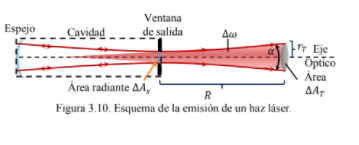
\includegraphics{Captura.PNG}
    \label{fig:my_label}
\end{figure}

Consideremos un láser que emite un flujo de $\phi = 5mW$ en un haz con un ángulo de divergencia $\alpha = 1.3 m rad$. La cavidad del láser está diseñada de forma que tiene una ventana de salida circular con área $\Delta A_s = \num{2.5 e -3} cm$.

\begin{enumerate}
    \item Determinar el ángulo sólido $\Delta \omega$ a partir de las variables mostradas en la figura, y calcular su valor. Se puede hacer uso de aproximaciones de ángulo pequeño.
    
    \textbf{Sol:}
    
    Otra expresión para el ángulo sólido que depende solamente de en este caso $\alpha$ es:
    
    \begin{equation*}
        \Delta \omega = 2 \pi (1 - \cos{(\alpha/2)})
    \end{equation*}
    
    \noindent y suponiendo que $\alpha << 1$ y usando la aproximación de segundo orden para coseno,
    
    \begin{equation*}
        \Delta \omega = 2 \pi (\cancel{(1 - 1)} +\frac{\alpha^2}{4}) = \pi \alpha^2/4 = \num{1.327 e-6} sr
    \end{equation*}
    
    \item Determinar la radiancia de salida del láser en unidades de $\left[\frac{W}{cm^2 sr}\right]$ y la irradiancia que cruza la ventana de salida en $\left[\frac{W}{cm^2}\right]$.
    
    \textbf{Sol:}
    Como la salida del láser se puede aproximar como un haz colimado, entonces la irradiancia se puede escribir como:
    
    \begin{equation*}
        I = \frac{\Phi}{\Delta \omega \Delta A_s} = 1507159 \frac{W}{cm^2 sr}
    \end{equation*}
    
     Al tener un flujo homogéneo, la irradiancia se puede describir solamente por el flujo y el área:
     
     \begin{equation*}
         I = \frac{\Phi}{\Delta A_s} = \frac{\num{5e-3}W}{\num{2.5 e-3}cm^2} = 2 \frac{W}{cm^2}
     \end{equation*}
    
    
    
    
    
    \item Si se tiene un radiómetro con área circular de $A_F = 5.244 mm^2$. ¿Cuál será la distancia máxima desde la ventana de salida en la que el láser pueda ser considerado como haz colimado? Argumentar la respuesta. Pista: Debido a la divergencia del haz desde su ventana de salida, se puede aproximar como proveniente de una fuente puntual detrás de la ventana y que solo emite luz en un ángulo sólido $\Delta \omega$. Considerar la relación de flujo de energía con las distintas áreas involucradas.
    
    \textbf{Sol:}
    
    Al ser $A_F$ circular,
    
    \begin{equation*}
        A_F = \pi r^2 \hspace{0.3cm} \rightarrow \hspace{0.3cm} r = \sqrt{\frac{A_f}{\pi}}
    \end{equation*}
    
    entonces tenemos un triangulo rectángulo donde el cateto opuesto es $r$, el cateto adyacente es la distancia de la ventana al radiómetro $R$ y el ángulo es $\alpha/2$ y así:
    
    \begin{equation*}
        \tg{\alpha/2} = \frac{r}{R} \hspace{0.3cm} \rightarrow \hspace{0.3cm} R = \frac{r} {\tg{\alpha/2}} =\sqrt{\frac{A_F}{\pi\tg^2{\alpha/2}}}  = 1988 mm
    \end{equation*}
\end{enumerate}



%%%4%%%



\item Suponga que se tiene un radiómetro con un área de $5.24 mm^2$ a una distancia de $1m$ de una fuente puntual con una potencia de $100W$, calcular lo siguiente:

\begin{enumerate}
    \item La intensidad radiante total emitida por la fuente.
    
    \textbf{Sol:}
    
    Suponiendo que se tenga un frente de onda esférico, la intensidad radiante total es:
    
    \begin{equation*}
        E = \frac{\Phi}{\Delta \omega} =\frac{\Phi}{\frac{A_S}{R^2}}= \frac{100 W}{4 \pi \cancel{(R^2/R^2)}} sr \approx 7.96 \frac{W}{sr}
    \end{equation*}
    
    \item La fracción del flujo de radiación que llega al radiómetro.
    
    Por el inciso anterior,
    
    \begin{equation*}
        \frac{\partial  \Phi}{\partial \omega} = \frac{100}{4 \pi} \frac{W}{sr}
    \end{equation*}
    
    \begin{equation*}
        d\Phi = \frac{100}{4 \pi} \frac{W}{sr} d\omega
    \end{equation*}
    
    que integrando,
    
    \begin{equation*}
        \Phi = \frac{100}{4 r^2 \pi} \frac{W}{sr} \iint  r^2\sin{\theta} d\theta d\phi
    \end{equation*}
    
    y como el area del radiómetro es de $\num{5.24e-6} m^2$ y está a una distancia de $1m$,
    
    \begin{equation*}
        \Phi = \frac{100}{4 (1m)^2 \pi} \frac{W}{sr} (\num{5.24e-6} m^2) = \num{4.17e-5} W 
    \end{equation*}
    
    \textbf{Sol:}
    
    \item La irradiancia medida por el fotodiodo en $W/m^2$
    
    \textbf{Sol:}
    
    Al tenerse una fuente puntual, la irradiancia depende solo del flujo $\Phi$ y área así que:
    
    \begin{equation*}
        I = \frac{\Phi}{A} = \frac{\num{4.17e-5}W}{\num{5.24 e-6}m^2} = 7.96 \frac{W}{m^2}
    \end{equation*}
    
    \item Repetir lo anterior cuando el radiómetro está a $2 m$ de la fuente.
    
    \textbf{Sol:} 
    
    En este caso el flujo es:
    
    \begin{equation*}
        \Phi = \frac{100}{4 (2m)^2 \pi} \frac{W}{sr} (\num{5.24e-6} m^2) = \num{1.04e-5} W 
    \end{equation*}
    
    entonces la irradiancia es:
    
    \begin{equation*}
        I = \frac{\Phi}{A} = \frac{\num{1.04e-5}W}{\num{5.24 e-6}m^2} = 1.98 \frac{W}{m^2} 
    \end{equation*}
\end{enumerate}

    
    
\end{enumerate}

\end{document}